%latex model.tex
%bibtex model
%latex model.tex
%latex model.tex
%pdflatex model.tex

%se poate lucra si online (de ex www.overleaf.com)


\documentclass[runningheads,a4paper,11pt]{report}

\usepackage{algorithmic}
\usepackage{algorithm} 
\usepackage{array}
\usepackage{amsmath}
\usepackage{amsfonts}
\usepackage{amssymb}
\usepackage{amsthm}
\usepackage{caption}
\usepackage{comment} 
\usepackage{epsfig} 
\usepackage{fancyhdr}
\usepackage[T1]{fontenc}
\usepackage{geometry} https://www.overleaf.com/project/5f81b795d430cc0001f50400
\usepackage{graphicx}
\usepackage[colorlinks]{hyperref} 
\usepackage[latin1]{inputenc}
\usepackage{multicol}
\usepackage{multirow} 
\usepackage{rotating}
\usepackage{setspace}
\usepackage{subfigure}
\usepackage{url}
\usepackage{verbatim}
\usepackage{xcolor}

\geometry{a4paper,top=3cm,left=2cm,right=2cm,bottom=3cm}

\pagestyle{fancy}
\fancyhf{}
\fancyhead[LE,RO]{Automated Assistant for medical students}
\fancyhead[RE,LO]{SocialGoodTeam}
\fancyfoot[RE,LO]{MIRPR 2020-2021}
\fancyfoot[LE,RO]{\thepage}

\renewcommand{\headrulewidth}{2pt}
\renewcommand{\footrulewidth}{1pt}
\renewcommand{\headrule}{\hbox to\headwidth{%
  \color{lime}\leaders\hrule height \headrulewidth\hfill}}
\renewcommand{\footrule}{\hbox to\headwidth{%
  \color{lime}\leaders\hrule height \footrulewidth\hfill}}

\hypersetup{
pdftitle={artTitle},
pdfauthor={name},
pdfkeywords={pdf, latex, tex, ps2pdf, dvipdfm, pdflatex},
bookmarksnumbered,
pdfstartview={FitH},
urlcolor=cyan,
colorlinks=true,
linkcolor=red,
citecolor=green,
}
% \pagestyle{plain}

\setcounter{secnumdepth}{3}
\setcounter{tocdepth}{3}

\linespread{1}

% \pagestyle{myheadings}

\makeindex


\begin{document}

\begin{titlepage}
\sloppy

\begin{center}
BABE\c S BOLYAI UNIVERSITY, CLUJ NAPOCA, ROM\^ ANIA

FACULTY OF MATHEMATICS AND COMPUTER SCIENCE

\vspace{6cm}

\Huge \textbf{AI assistant for a prostate medicine student}

\vspace{1cm}

\normalsize -- ITSG report --

\end{center}


\vspace{5cm}

\begin{flushright}
\Large{\textbf{Team members}}\\
Bocsa Mirela Alexandra, Software Engineering, 258, bmis2033@scs.ubbcluj.ro

Roman Adrian, Software Engineering, 258, rais2087@scs.ubbcluj.ro

Vaida Andrei Lucian, Software Engineering, 258, vais2096@scs.ubbcluj.ro

Vrincean Alexandru, Software Engineering, 258, vais2100@scs.ubbcluj.ro
\end{flushright}

\vspace{2cm}

\begin{center}
2020-2021
\end{center}

\end{titlepage}

\pagenumbering{gobble}

\begin{abstract}
	

Prostate cancer is the most common cancer among men and is the second leading cause of cancer death in men after lung cancer.In the last few years, In the medical system, the amount of data that needs to be analyzed has increased dramatically, which means that much more effort is needed from doctors and experts. Therefore, an intelligent algorithm capable of detecting the cancer prostate is needed.\par
In order to solve this problem, we proposed two UNET models that will learn to detect the possible cancer zone from a medical image. Both models follow the classical UNET architecture, what is different are the number of features  per layer.\par
The dataset contains about 900 slices from 30 patients. Because of this small number of input data and due the fact that the images are very dark, with a lot of noise and just a small part of them represents the prostate and even a smaller one describes the cancer area, the results are quite disappointing. The UNets didn't manage to learn and identify, neither the prostate, nor the cancer area. \par
Even if the results are not very satisfying and the U-Net models are not yet able to detect the prostate cancer zone very accurately, they still prove that a U-Net can be used for prostate cancer segmentation. With more training time and more competent hardware, if the number of epochs and the batch size is increased, as well as the original size of the input images is kept, and a better preprocessing of the input data, the result may improve and the models will be able to accurately detect the prostate cancer zone.\par
\end{abstract}


\tableofcontents

\newpage

\listoftables
\listoffigures
\newpage

\setstretch{1.5}

\newpage
\textbf{Team contribution:\newline}\par

\textbf{Bocsa Mirela:}
\begin{itemize}
	\item Intelligent algorithm research, dataset acquisition and dataset processing
	\item Prepare the input for the neural network, implement the 2 UNET models, train the algorithm, play with the parameters
	\item Analyze result
	\item Update documentation
\end{itemize}

\textbf{Roman Adrian:}
\begin{itemize}
	\item Server and client implementation
	\item Dataset researching
	\item Update documentation
\end{itemize}

\textbf{Vaida Andrei Lucian:}
\begin{itemize}
	\item Application basecode, client-server architecture and implementation
	\item Dataset researching and acquisition, training attempts
	\item Update documentation and video presentation
\end{itemize}

\textbf{Vrincean Alexandru:}
\begin{itemize}
	\item Server and client implementation
	\item Continuous feedback of teamwork
\end{itemize}

\newpage

\pagenumbering{arabic}


\chapter{Introduction}
\label{chapter:introduction}

\section{What? Why? How?}
\label{section:what}

Prostate cancer is the most common cancer among men and is the second leading cause of cancer death in men after lung cancer. The condition usually develops very slowly and mainly affects older men. About 6 out of 10 cases are diagnosed in men over 65, the disease being rarely detected before 40 years. The average age at diagnosis is approximately 66 years. The choice of appropriate treatment depends on several factors, including the stage of the disease, the patient's age, possible previous treatment options and last but not least the patient's preferences.\cite{reginaMaria}

In the medical system, the people responsible for interpreting medical data are only medical experts. But, in the last few years, the amount of data that needs to be analyzed has increased dramatically, which means that much more effort is needed from doctors. Furthermore, the interpretation of medical data performed by a medical expert is due the level of expertise of the person that reads the data, to its subjectivity and the complexity of the image.

Therefore, we propose an application that will allow a student to upload a medical image of a prostate organ, visualize it and, with the help of an intelligent algorithm, tell him if that prostate is suspected of cancer or not. The application will display a new image with a frame surrounding the location of the possible tumor.

Machine learning algorithms come with a big help in medical data analysing since they are capable of interpreting very big images and providing an accurate and efficient diagnosis. Moreover, there will be no subjectivity involved and, unlike humans, the algorithm will not get tired, on the contrary, the more data received, the more accurate the result will be.\cite{imageProcessing}

\section{Paper structure and original contribution(s)}
\label{section:structure}

The research presented in this paper advances the theory, design, and implementation of several particular models. 

The main contribution of this report is to present an intelligent algorithm for solving the problem of prostate cancer detection from a medical image.

The second contribution of this report consists of building an intuitive, easy-to-use and user
friendly software application. Our aim is to build an application that will help a medical student to identify and monitor cancer cells from a prostate medical image. This is done in a user friendly-manner, but with all the support of the accuracy of an intelligent algorithm.

The third contribution of this thesis consists of the new results obtained by our intelligent algorithm comparing them with the results obtained by other similar algorithms.


The present work contains $xyz$ bibliographical references and is structured in five chapters as follows.

The second chapter/section describes the problem definition and the representation of our data.

The chapter \ref{chapter:stateOfArt} details  the related work and state-of-the-art results of the methods utilised until now in order to solve the given problem.

The chapter \ref{chapter:proposedApproach} details our approach and offers more details about the algorithm we use to address the problem. 

The chapter \ref{chapter:applicationRequirements} introduces our application and its main functionalities from the user perspective and also describes the tools and technologies we used for building the application.

The chapter \ref{chapter:application} explains the experimental methodology and the numerical results obtained with our approach and the state of art approaches. Our focus in this chapter is on the interpretation and the statistical validation of the results.

In the end, in the chapter \ref{chapter:concl} we summarize our conclusions and future work and also try to analyze the strengths and weaknesses of our application with the focus on what we can improve both in the algorithm and the application.


\chapter{Scientific Problem}
\label{section:scientificProblem}


\section{Problem definition}
\label{section:problemDefinition}

The goal of this project is to help medicine students to study prostate cancer by providing them an application in which they can load an image an receive a result with the zone of the possible prostate tumor. Students can use the application to apply the theoretical notions learned in the courses.

In recent years, prostate cancer has become more common such that it is estimated that one in six men will develop prostate cancer in their lifetime. Although the prostate cancer is usually not the direct cause of death, the differentiation of clinically
significant prostate cancer lesions from those low-grade lesions is critical. The state-of-the-art diagnostic method uses multiparameteric MR imaging with transrectal
ultrasound-guided biopsy. This method is the most accurate imaging method for prostate cancer detection, but, it requires
the expertise of experienced radiologists, and as such, there is inconsistency across readers of varying experience. In order to reduce the rate of occurrence of errors due to inattention or the medical judgment, subjectivity and level of expertise, an intelligent algorithm that can detect the prostate cancer is needed.\cite{multiparametric} 

The main advantage of an artificial intelligent algorithm is its ability to analyse and employ an enormous quantity of data, much more efficiently than possible for humans through classical statistical analyses. Moreover, the more data received, the more accurate the result will be. There will be no more subjectivity involved and less high level of prostate cancer expertise will be required.\cite{imageProcessing}

On the other hand, processing medical image is a challenge even for an intelligent algorithm. Most of the prostate image may be difficult to read an interpret, which means that large sets of data with labeled images are required for the algorithm to work properly. Machines are still having a hard time understanding medical images and using certain unclear images can be misleading for the AI, that can provide erroneous or implausible detections.

The following sections will describe the input and the output set.

\section{Input }
\label{section:input}

The input for the intelligent algorithm will be a set of medical images containing from 26 to 30 slices with the prostate MRI of a specific patient. These images may or may not represent a prostate with possible cancer zones. Each slice has 512x512 pixels.

\section{Output }
\label{section:output}
The output that the intelligent algorithm will provide will be a new medical image with the segmentation of the prostate and the possible prostate cancer zones.


\chapter{State of the art/Related work}
\label{chapter:stateOfArt}
To solve problems similar to ours, the literature describes the way deep convolution neural networks are used.
The success of the most used approaches is based on the fact that lately there have been developed more powerful graphics processing units and the big number of annotated images that appeared. Helpful was also the fact that there were developed many classification \cite{imagenetClassification}, object detection \cite{largeScaleImageRecognition} and even segmentation \cite{semanticSegmentation} algorithms.\par 
The success of segmenting an image is determined by the edge detection in different contexts. This is why a lot of work consisted in finding the edge's features.\cite{zhang2015ensemble} Fortunately, it is believed that deep learning can effectively learn edge features.\par

As described above, many researchers have utilized deep learning in medical image analysis. With the advance of deep learning, these methods obtained outstanding performances. Considering these results, the medical imaging research community started manifesting interest for deep learning-based methods used to detect cancer. In the following sections, two approaches used for prostate cancer detection will be described, with the focus on the results they obtained.

\section{U-Net for Prostate Segmentation}
\label{section:CNNApproach1}

This approach uses a U-Net
which, trained end-to-end, can segment the prostate on MR images accurately and fast. The neural network architecture they used is a classical U-Net, but with some additional improvements to combat overfitting and all the  challenges the prostate images came with.

\subsection{Algorithm}
\label{section:algorithm}

The proposed U-Net neural network contains three parts. The first five stages consist of a compression path which extract features from the data and reduce the resolution by an appropriate stride. From top to the fourth stage, the number of feature channels is doubled at each stage. In the first stage, the number of feature channels is
64, which means that the last stage will have 512 feature channels. In each stage, a 3x3 convolutions and one 1x1 convolution are performed, followed by one 2x2 max pooling operation for down sampling. On the contrary, the later four stages consist of an expansive path which upsample the features maps and halve the number of feature channels until its original size is reached. These stages have same operations like the stage within compression path except the max pooling operation. On the part of supervised layers, each supervised layer consists of a upsampling layer and a deconvolution layer. The upsampling layer upsamples the features map and then via deconvolution layer obtain the segment result. During training, these supervised layers control
the process of training according to the difference between segmentation result and ground truth.

A standard
stochastic gradient descent with Dice coefficient were used as a loss function.
 \cite{deeplySupervisedCNN}

\subsection{DataSet}
\label{section:dataset}

The model was trained on a dataset containing 1324 images that came form 81 patients. The images was acquired using a Philips 3T MRI scanner and were grouped in volumes consisting of 26 slices, each slice having 512x512 pixels. Because of this small number of data, in order to increase the robustness, reduce overfitting and  enlarge the training dataset, the data augmentation strategy was employed by applying translations, rotations and zooms.\cite{deeplySupervisedCNN}

The ground truth and result of segmentation were binary images with the possible location of the cancer zone. \cite{deeplySupervisedCNN}

\subsection{Results}
\label{section:results}

In order to evaluate the model, 4
patients with 64 images were randomly chosen before training to take part of the evaluation dataset. To evaluate the algorithm the Dice coefficient was used. The obtained results are described in Table \ref{tab1Results}. These results prove that, comparing with a FCN or a simple U-Net, the proposed approach obtained better score, showing that the proposed method is a viable method for improving neural network's performances for medical images segmentation.\cite{deeplySupervisedCNN}

\begin{table}[htbp]
		\begin{center}
			\begin{tabular}{p{180pt}c c c c}
				\textbf{Method}&\textbf{meanDSC}& \textbf{medianDSC}&\textbf{maximumDSC} \\
				\hline\hline
 			Approach method& 0.885& 0.945& 0.985 \\
 			U-Net& 0.865& 0.940& 0.969 \\
 		    FCN& 0.759& 0.832& 0.918 \\
			\end{tabular}
		\end{center}
		\caption{Comparison between the proposed approach and other methods \cite{deeplySupervisedCNN}}
		\label{tab1Results}
\end{table}

\section{Prostate Cancer Detection using Deep Convolutional Neural Networks}
\label{section:CNNApproach2}

This approach proposed an automated pipeline for two levels of prostate cancer classifcation: slice level and patient level. For slice-level classifcation, a stack of individually trained modifed ResNet CNNs are used. In order to convert slice-level classifcation results into patient level, this paper came with first-order statistical features extractor, a decision tree-based feature selector and a Random Forest classifer. The obtained results seems to be  more robust compared to similar studies that proposed CNNs for prostate cancer detection. \cite{deepCNN}

\subsection{Algorithm}
\label{section:algorithm}

The base architecture for this research is a ResNet architecture. Each Residual block consists of convolutional layers and identity shortcut connection that skips those layers and their outcomes are added at the end. In order to boost the performance of the architecture, a fully pre-activated residual network is implemented by applying  batch normalization and ReLU activation layers before the convolution layers. Instead of using the classical 2-layer deep ResNet block, the method this paper proposed uses a 3-layer deep bottleneck building block because of the fact it will reduce the training time without sacrificing the performance. The ResNet neural network is a 41 layers deep network. The architecture is composed of 2D convolutional layers with a 7 x 7 filter and a 3 x 3 Max pooling layer and residual blocks. Since the input images were small and the tumorous regions were even smaller, additional ResNet blocks were needed. Te first ResNet block is 3-layer bottleneck blocks with 2D CNN layers with (64, 64, 256) filter size. It will be stacked 4 times. Te second ResNet Block is 3-layer bottleneck blocks with 2D CNN layers with (128, 128, 512) filter size. This one will be stacked 9 times. At the end of the Res Blocks a 2 x 2 Average pooling, a dropout layer and 2D fully connected layer are applied. The optimizer this method used was a Stochastic Gradient Decent one with Binary Cross Entropy as the loss function.\cite{deepCNN} The parameters used to train the neural network are describe in Table \ref{tableParameters}.
The output of each ResNet will consist of two probabilities associated with each class (PROSTATE CANCER and NON PROSTATE CANCER) for each DWI slice.

\begin{table}[htbp]
		\begin{center}
			\begin{tabular}{p{180pt}c c c c}
				\textbf{Parameter}&\textbf{Value}\\
				\hline\hline
 			Initial learning rate& 0.001\\
 			LR reduce factor& 10\\
 			Batch size& 8\\
 			Dropout rate& 0.9\\
 			Weight decay& 0.000001\\
 			Momentum& 0.9\\
			\end{tabular}
		\end{center}
		\caption{ResNet Parameters \cite{deepCNN}}
		\label{tableResults}
\end{table}

\subsection{DataSet}
\label{section:dataset}

The data was acquired using using a Philips Achieva 3T from 427 patients. From these 427 patients, 175 patients had clinically significant prostate cancer and 252 patients did not. From all this images, a total of 5,832 2D slices were obtained coming in DWI format. In order to use DWI images as input for the neural network, each slice was resized to 144 x 144 pixels and center cropped with 66 x 66 pixels such that the prostate was covered. The CNNs were modified to feed DWI data with 6 channels instead of images with 3 channels. In order to test the algorithm on a different data, all the DWI images were separated into three different sets, the training set with 271 patients consisting of 3,692 slices, the validation set with 48 patients containing 654 slices and the test set with 108 patients with 1,486 slices. Before using this images as input for the neural network, they were all normalized.\cite{deepCNN}

\subsection{Results}
\label{section:results}

In order to evaluate the performance of the proposed method, the AUC (area under the curve) and ROC (receiver operating characteristic curve) curve were used. The ROC curve plots true positive rates and false positive rates with different thresholds, while an AUC described the performance of the algorithm with a single number. Regarding the slice-level performance, the best AUC score was obtained by the first CNN, but the other 4 also come with great results. When talking about patient-level performance, the CNN worked also very well.\cite{deepCNN} All of these results are illustrated in Table \ref{tableResults}.

\begin{table}[htbp]
		\begin{center}
			\begin{tabular}{p{180pt}c c c}
				\textbf{Slice-level CNN}&\textbf{AUC}&\textbf{Confdence Interval}\\
				\hline\hline
 			CNN1& 0.87& 0.84-0.90\\
 			CNN2& 0.87& 0.83-0.90\\
 			CNN3& 0.86& 0.83-0.89\\
 			CNN4& 0.85& 0.82-0.88\\
 			CNN5& 0.85& 0.82-0.88\\
 			\\
 			\textbf{Patient-level CNN}&\textbf{AUC}&\textbf{Confdence Interval}\\
			\hline\hline
 			CNN& 0.84& 0.76-0.91\\
			\end{tabular}
		\end{center}
		\caption{ResNet Results \cite{deepCNN}}
		\label{tableParameters}
\end{table}
The obtained results seems to have a superior and a more robust performance compared to similar studies that proposed CNNs for prostate cancer detection.
\chapter{Investigated approach}
\label{chapter:proposedApproach}

\section{U-Net architecture }
\label{section:network}

The approach we used for detecting the prostate cancer is a convolutional network architecture. More precisely, it is a UNet with 3 sections: the contraction, the bottleneck and the expansion. All the convolutional layers were build in a 2D format to fit the input dataset format.

\subsection{U-Net Model 1}
\label{section:model1}
The contraction section is made of 4 contraction stages. The first stage will start with 64 filters. This number doubles after each block so that the neural network can learn the complex structures effectively, which means that the second stage will have 128 features, the third one will go with 256 and the last one will end up with 512 filters. For each stage, two convolutions with 3x3 kernel size are performed, one 1x1 convolution for the output and a 2x2 max pooling is attached for down sampling. Also, after some convolutions, dropout is also performed. Each 3x3 convolution uses RELU as activation function and the 1x1 convolution will use SIGMOID as activation function.

The bottleneck layer mediates between the contraction layer and the expansion layer. This will have 512 features channels and only two 3x3 convolutions and the 1x1 convolution are performed, with no max pooling. 

The expansion layer consists of several expansion stages. Each stage of this part includes two kinds of operations. The first one is upsampling which makes the size of feature map increase gradually until it reaches the size of the original input image and the second one is deconvolution (Deconv2D). This operation is used to halve the number of feature channels, so that the number of convolution kernels will be halved after each stage to maintain symmetry. However, because some image information will be lost after every convolution, the features extracted from early stages are get appended by features of the corresponding expansion layer. This action would ensure that the features that are learned while contracting the image will be used to reconstruct it. The number of expansion and contraction stages is the same (see Figure \ref{unet_architecture1}). \par 

\begin{figure}[!h]
	\centerline{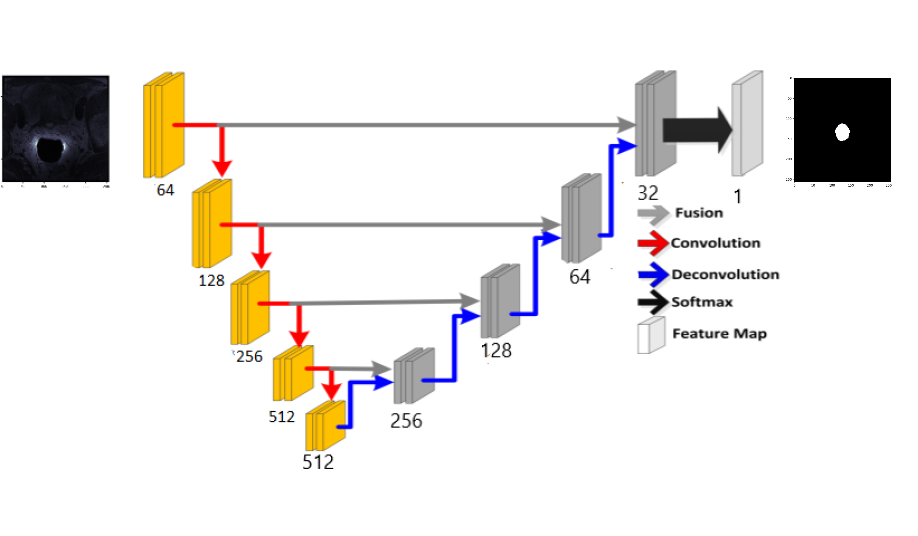
\includegraphics[width=20cm, height=12cm]{images/Unet_model1.png}}  
	\caption{U-Net(Model 1) Architecture}
	\label{unet_architecture1}
\end{figure}

\subsection{U-Net Model 2}
\label{section:model1}

The second U-Net architecture is similar with the previous one, but the number of filters at each stage is reduced. The first stage of the contraction section will start with 16 filters. This number is also doubled after each block so that the neural network can learn the complex structures effectively, which means that the second stage will have 32 features, the third one will go with 64 and the last one will end up with 128 filters. Two convolutions with 3x3 kernel size, one 1x1 convolution for the output, a 2x2 max pooling and a dropout are performed for each stage. The activation function used for this model is RELU, excepting for the last layer which will use SIGMOID.

The bottleneck layer will have 256 features channels and only two 3x3 convolutions and the 1x1 convolution are performed, with no max pooling. 

The expansion layer consists of 4 expansion stages. Each stage of this part includes upsampling and deconvolution(Conv2DTranspose). The number of filters starts from 128 for the most bottom layer and decreases until it reaches the same size as the first stage from the contraction stage, ending up with 16 filters. (see Figure \ref{unet_architecture2}). \par 

\begin{figure}[!h]
	\centerline{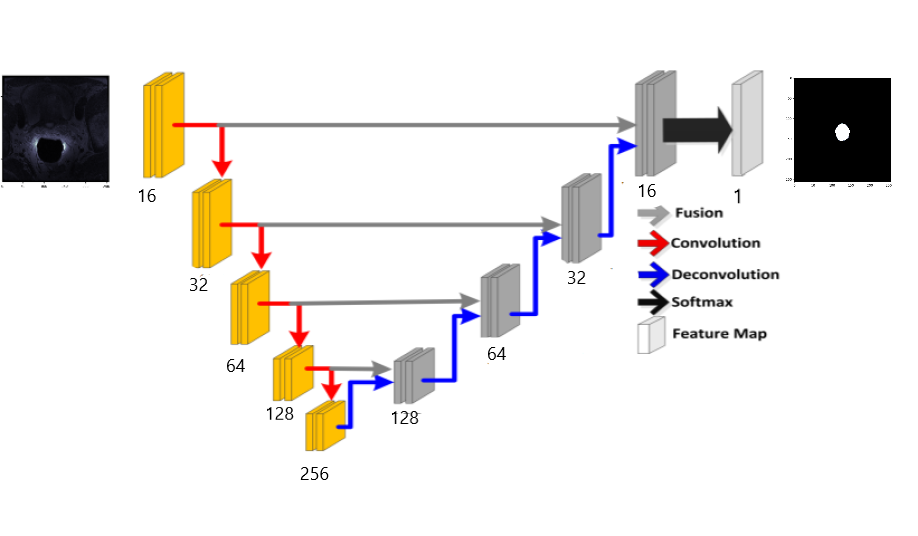
\includegraphics[width=20cm, height=12cm]{images/Unet_model2.png}}  
	\caption{U-Net(Model 2) Architecture}
	\label{unet_architecture2}
\end{figure}

\section{Model evaluation }
\label{section:evaluations}
During training, the supervised layers control the process of training according to the difference between segmentation result and ground truth. In order to measure this difference, we used DICE coefficient, which is essentially a measure of overlap between two samples. The values of the DICE coefficient ranges from 0 to 1 where a Dice coefficient of 1 denotes perfect and complete overlap. \par

\[DICE = \textstyle\frac{2\times{|A \cap B|}}{|A|+|B|}$\]

Where \cite{dice}:
\begin{itemize}
	\item |A \cap$ B| = the common elements between sets A and B
	\item |A| = the number of elements in set A
	\item |B| = the number of elements in set B
\end{itemize}

Because we have to apply the DICE coefficient on segmentation masks, in order to evaluate the \newline  |A \cap$ B| an element-wise multiplication between the prediction and target mask was applied followed by the sum of the resulting matrix. The loss function that will be used by the neural network will be \newline \boldsymbol{1 - DICE}.

\section{Implementation details }
\label{section:implementation}
For implementing the UNet we used Keras with Python. As layers we used Conv2D, Deconv2D and Conv2DTranspose, as well as MaxPooling2D and Dropout. The neural network will receive the following parameters:
\begin{itemize}
	\item Optimizer: Adam
	\item Learning rate: 0.001
    \item Momentum: 0.9
	\item Dropout: 0.3
	\item Batch size:2
	\item Number of epochs: 250
\end{itemize}

\section{Dataset}
\label{section:dataset}
The dataset had very limited number of images, only 30 patients with 2 examinations which means a total of 60 volumes. Each volume has from 26 to 30 slices, so the final dataset contains 890 slices.  Because of this small number of data, the model resulted suffering from overfitting. To increase the
robustness and reduce overfitting, we adopted the strategy of data augmentation to enlarge the training dataset. The augmentation transformations include translation, rotation and
zoom. Before feeding the model with the input dataset, all the images were normalized and the pixel values were reduced to [0-1] interval. \par
In order to train and evaluate the model, we chose 75\% of the total images for training and the rest for evaluation. We also excluded 1 patient from the dataset in order to use it for testing the model.\par
Below is an example of an input image and the corresponding prostate mask as well as the input and the corresponding cancer zone:\par
\begin{figure}[!h]
\centering
  \begin{minipage}[b]{0.4\textwidth}
    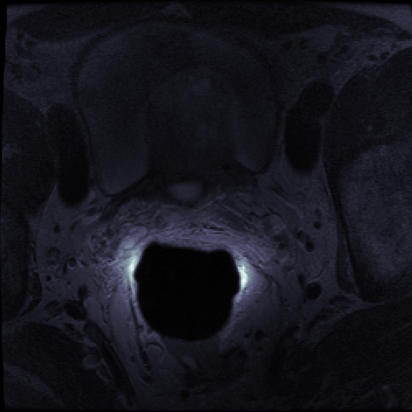
\includegraphics[width=\textwidth]{images/input_prostate.png}
    \caption{Input}
  \end{minipage}
  \begin{minipage}[b]{0.4\textwidth}
    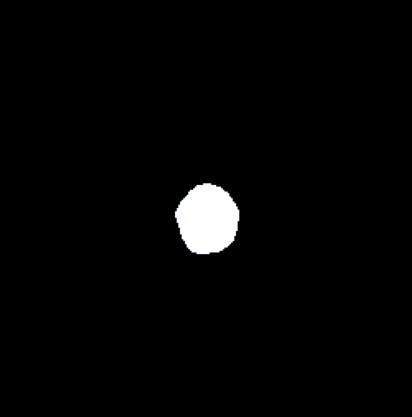
\includegraphics[width=\textwidth]{images/mask_prostate.png}
    \caption{Mask (whole prostate)}
  \end{minipage}
\end{figure}

\caption{Caption for this figure with two images}
\label{fig:image2}
\end{figure}

\begin{figure}[!h]
\centering
  \begin{minipage}[b]{0.4\textwidth}
    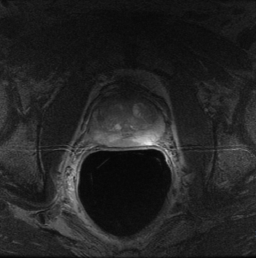
\includegraphics[width=\textwidth]{images/input_cancer.png}
    \caption{Input}
  \end{minipage} 
  \begin{minipage}[b]{0.4\textwidth}
    
\includegraphics[width=\textwidth]{images/mask_cancer.png}
    \caption{Mask (cancer zone)}
  \end{minipage}
\end{figure}

\caption{Caption for this figure with two images}
\label{fig:image2}
\end{figure}

\chapter{Application Requirements}
\label{chapter:applicationRequirements}

\section{Application main functionalities}
\label{section:functionalities}

The main functionalities of the application we developed are the following: 
\begin{itemize}
	\item The system should allow the user to upload a medical image that is a representation of the prostate organ
	\item The system should display the medical image the user has uploaded
	\item The system should allow the user to check if the medical image has a prostate cancer zone
	\item The system should allow the user to visualize the prostate cancer zone
	\item The system save the images that the user uploaded
	\item The system should allow the user to visualize again the images that he uploaded
\end{itemize}

\section{Tools and Technologies}
\label{section:toolsAndTechnologies}

In order to provide to students an easy way to access the application, we developed a web application based on a Python server and a React web client.

The Python server: The server side was written in Python using Keras for the neural network, a generator for applying different transformations on the input images and pydicom and numpy libraries for preparing the input dataset.\par
The React client was developed using TypeScript and the new Hooks technology.
React is a declarative and component-based JavaScript library for efficiently building interactive user interfaces. It uses encapsulated components that manage their own state, then compose them to make complex UIs.\cite{react}
TypeScript is an open-source language which builds on JavaScript, by adding static type definitions. This allow the developers to better understand the code, makes it more readable and thus it reduces errors.
Hooks are a new addition in React 16.8. They let you use state and other React features without writing a class\cite{reactHooks}. Hooks technology allowed us to develop lighter and more readable components by using hooks like \emph{useState()}, so we could update our components without taking care to update the sensitive state of the components as was done before. Furthermore, we didn't used the classic stateful class component, but the stateless functional components, which are plain JavaScript functions that returns JSX and are easier to develop.
To create requests to the server we used Axios, a promise based HTTP client.

Even if our client application is, for now, a simple image uploader and downloader, we created a scalable architecture by creating a generic HTTP service which is used by a custom service for our images, which is used by our UI component.

In order to display medical images (like DICOM and NIFTI), we used the Med3Web library, a high performance web tool for advanced visualization medical volumetric (both in 2d and 3d modes). The latest version can be used with WebGL-enabled desktop browsers (Chrome, Firefox, Opera) and allow limited usage with mobile browsers (Android Chrome). Version for Safari (macOS, iOS) is planned for future.\cite{Med3Web} Because medical images can be very dark, one of the advantages of this library is that the user is allowed to change the brightness of uploaded images in order to see them better. Even if they are not mandatory for our application, other features like drawing over the image or calculating distances between two points are available.


\chapter{Application (numerical validation)}
\label{chapter:application}

\section{Methodology}
\label{section:methodology}
	In order to evaluate our method we used the DICE coefficient, which measures the overlap between the input and the mask. We also output the accuracy, but the model didn't take it into consideration as part of the loss calculation.
	We trained our model 2 times, one for the prostate segmentation and the other one for the cancer zone. The aim is to predict the location of the prostate and the cancer zone and in order to display these 2 segmentations over the original image. In this way, a student can better analyze and study the prostate and the possible tumor.  \par
	The dataset used for training corresponds to real prostate images collected from 30 patients. These images are medical images and come in a DICOM format representing the axial, T2-weighted magnetic resonance imaging of the patient prostate. This dataset was a great challenge for our model since all the images were very dark, with lack of clear boundary specifically at the apex and base and a huge variation of shape and texture between the images from different patients. We also had to resize the images at half of their dimension which made it even more difficult for the neural network to learn and to be able to predict the prostate/cancer zone. The methods described in the Related Work \ref{chapter:stateOfArt} section used different datasets than our model. For instance, in  \cite{deeplySupervisedCNN}, the dataset contained over 1200 images, but, most important, the quality of the these images was better. They were lighter and there was not so much noise, which helped the model to learn faster and more accurate. The second approach\cite{deepCNN} presented as related work, had even more slices in the dataset. There were about of 5,832 2D slices, way more than 890 that we used.
	

\section{Data}
\label{section:data}

\subsection{Data acquisition}
\label{section:data_acquisition}

The training and testing data were taken from an online database provided by the \textbf{\textit{The Cancer Imaging Archive (TCIA) Public Access}}. All of the imaging studies were acquired at 3 Tesla magnet strength. Due to the scanner hardware upgrade in the middle of the study, 6 of the patients had baseline and repeat study performed on a GE Signa HDxt platform, while the remaining 7 patients were scanned on a GE Discovery MR750w. Transrectal coil within an air-filled balloon was used in all imaging studies. mpMRI protocol included T2-weighted, Diffusion Weighted (DW) and Dynamic Contrast Enhanced (DCE) sequences.
The imaging data is accompanied by the following types of derived data: manual segmentations of the total prostate gland, peripheral zone of the prostate gland, suspected tumor and normal regions (where applicable). Segmentations were done by a radiologist with the expertise in prostate MRI
volume measurements (for axial T2w images and ADC images) and mean ADC (for ADC images) corresponding to the segmented regions. Type of cancer: confirmed or suspected prostate cancer.\cite{dataset}

\subsection{Data storage}
\label{section:data_storage}

The data used for training and evaluating the model is stored locally, on the development server, in a folder called \emph{data} with 2 subfolders, \emph{input} and \emph{mask}. Additionally, when using a data generator, the preprocessed images are also stored on the local development server, in a npy format such as, the next time the model will be trained there will be no need to preprocess and load the dataset again. In this situation, the already npy saved data will be used.\par
For the data the student will want to analyze, he/she needs to press the \emph{Select image(s) to analyze} button and to select a Nifti image or one or more DICOM slices. The application will upload the image(s) to the server. The server will analyze the file(s) and will return a ZIP archive containing a DCM file, representing the prediction, for each image provided by the student.
In the current stage of development, these images are stored only until the next request from a user, so they are not persisted. As future work we want to add the possibility for the student to create a personal account through which it can be saved all his/her uploaded images and their predictions.

\subsection{Data visualisation}
\label{section:data_visualisation}
During training, we wanted to visualize the input data, but more over, the predicted output of the model we built. In order to be able to do that, we used \textbf{Pyplot} form \textbf{\textit{Matplotlib}} library which works very well with numpy arrays that we used for defining the input for our neural network. The predicted output will also be a numpy array. Therefore, by using \textbf{Pyplot} we managed to display and analyze the neural network prediction.\par
On the client side, the student have two possibilities to visualize medical images, by pressing the \emph{Open} button: loading from computer and loading from an URL. It can be selected a single file or multiple files, if the image is a DICOM with multiple slices. Before displaying the selection, the application shows a small window with the selected image (or the middle one if the student selected multiple slices) and prompts the user to confirm and adjust the luminosity of the image; more exactly the lower bound of the dark pixels and the upper bound of the white pixels. This is a very helpful feature of the Med3Web library since some medical images are very dark and has to be brighter so that they can be easily seen by human.
After loading the images into the web client, the user can change the plane (slice) view (thus, the library automatically detects the appropriate display method) and interactively visualize each slice of the image by dragging a slider.
Furthermore, in the top-left corner of the image are displayed some information about the image, like it's resolution, and, by selecting the \emph{Get voxel intensity} tool, each click on the image will display the coordinates of that point, in 3D. The application allows a user to create an account and login with that account to save his image(s), including predictions on the server. He can then see them displayed in a list  organized by dates.
\section{Results}
\label{section:results}

As mentioned before, the dataset used for training and testing the model consists of 890 2D slices: 645 for training, 215 for validation and 30 (1 patient) for testing. We built 2 UNets, with the same hyper-parameters that we previously described, but with different architecture. For both the models, we used generator for building the input data, which means that the input will also be the same. Both models were describe in \ref{chapter:proposedApproach}.\par
In the following sections, we will describe the results obtained by this two models, comparing them with the results obtained by other approaches that solved the same problem of prostate cancer segmentation.

\subsection{Model 1 results}
\label{section:unet1_results}

The first model we used is a 2D Unet, having \textbf{[64, 128, 256, 512, 512, 512, 256, 128, 64, 32]} number of features per convolutional layer and the input/output image size of 256X256.\par
After 100 epoch, the results are quite disappointing. The DICE coefficient reached a value of only \textbf{0.0023}. Even if we let our model run for 250 epoch, the results are the same, the DICE coefficient didn't reach any improvements. Moreover, due the huge the number of features per convolutional layer, the time required by the UNet to complete an epoch was about \textbf{5 mins}.\par
The results are illustrated in Fig \ref{epoch_dice_coef_model1} and Fig \ref{epoch_loss_model1}.

\begin{figure}[!h]
	\centerline{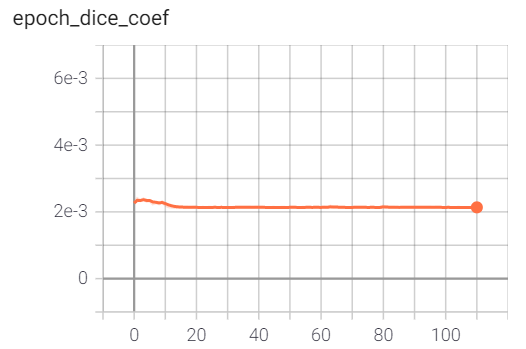
\includegraphics{images/epoch_dice_coef_model1.PNG}}  
	\caption{Epoch DICE coefficient (x: number of epochs, y: DICE coefficient value)}
	\label{epoch_dice_coef_model1}
\end{figure}

\begin{figure}[!h]
	\centerline{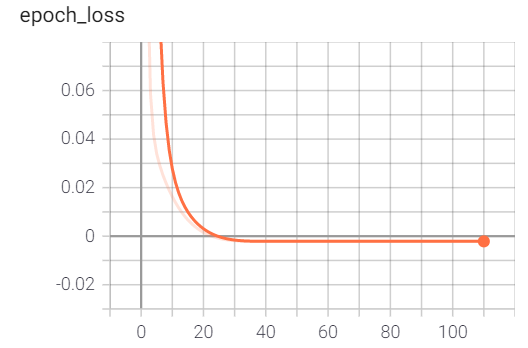
\includegraphics{images/epoch_loss_model1.PNG}}
	\caption{Epoch loss (x: number of epochs, y: loss value)}
	\label{epoch_loss_model1}
\end{figure}

\subsection{Model 2 results}
\label{section:unet2_results}

The second model we used is also a 2D Unet, but, with \textbf{[16, 32, 64, 128, 256, 256, 128, 64, 32, 16]} number of features per convolutional layer and the same input/output image size of 256X256.\par
The number of epochs was also 250, but the results are very different comparing with the previous model. With this UNet, the DICE coefficient started from a value of \textbf{0.22} and after 10 epochs reached a value of \textbf{0.78}. The problem is that, even after the 250 epoch, it remains almost the same. With each new epoch completed this value changed just a little bit, remaining between 0.78 and 0.80, while the \cite{deeplySupervisedCNN} obtained a maximum DICE value of \textbf{0.985}. The model used smaller number of features per layer, which led to shorter time required for completing an epoch. This time, only \textbf{about 50 seconds} were need to complete an epoch.
Even if the DICE=0.80, the output segmentation is still mostly black. The results are illustrated in Fig \ref{epoch_dice_coef_model2} and Fig \ref{epoch_loss_model2}.\par

\begin{figure}[!h]
	\centerline{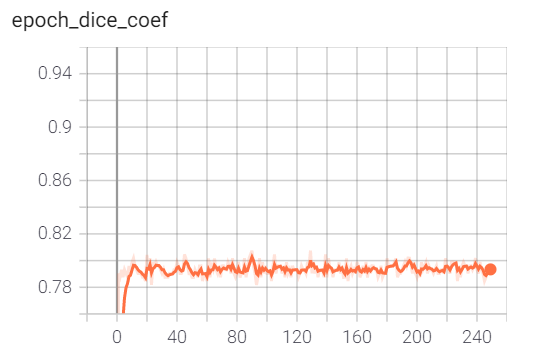
\includegraphics{images/epoch_dice_coef_model2.PNG}}  
	\caption{Epoch DICE coefficient (x: number of epochs, y: DICE coefficient value)}
	\label{epoch_dice_coef_model2}
\end{figure}

\begin{figure}[!h]
	\centerline{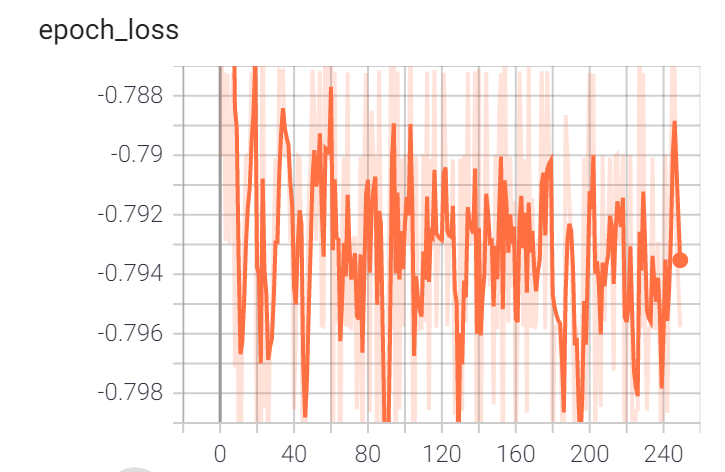
\includegraphics{images/epoch_loss_model2.PNG}}
	\caption{Epoch loss (x: number of epochs, y: loss value)}
	\label{epoch_loss_model2}
\end{figure}

\newline
Some small improvements we tried to implement were to use  \textbf{binary-crossentropy} as loss function and  \textbf{crop} the input images in order to eliminate the unnecessary information from each slice and increase the number of pixels of prostate zone.\par
The results we obtained with these changes and by using Model 2 are different than the previous ones. The dice coefficient 
started from a value of \textbf{0.0037} and the maximum value it reached was \textbf{0.05}. The loss value was \textbf{0.161} after the first epoch and in the end (after 20 epochs) it increased up to \textbf{0.0221}. These results are illustrated in the logs below(Fig \ref{logs}):

\begin{figure}[!h]
	\centerline{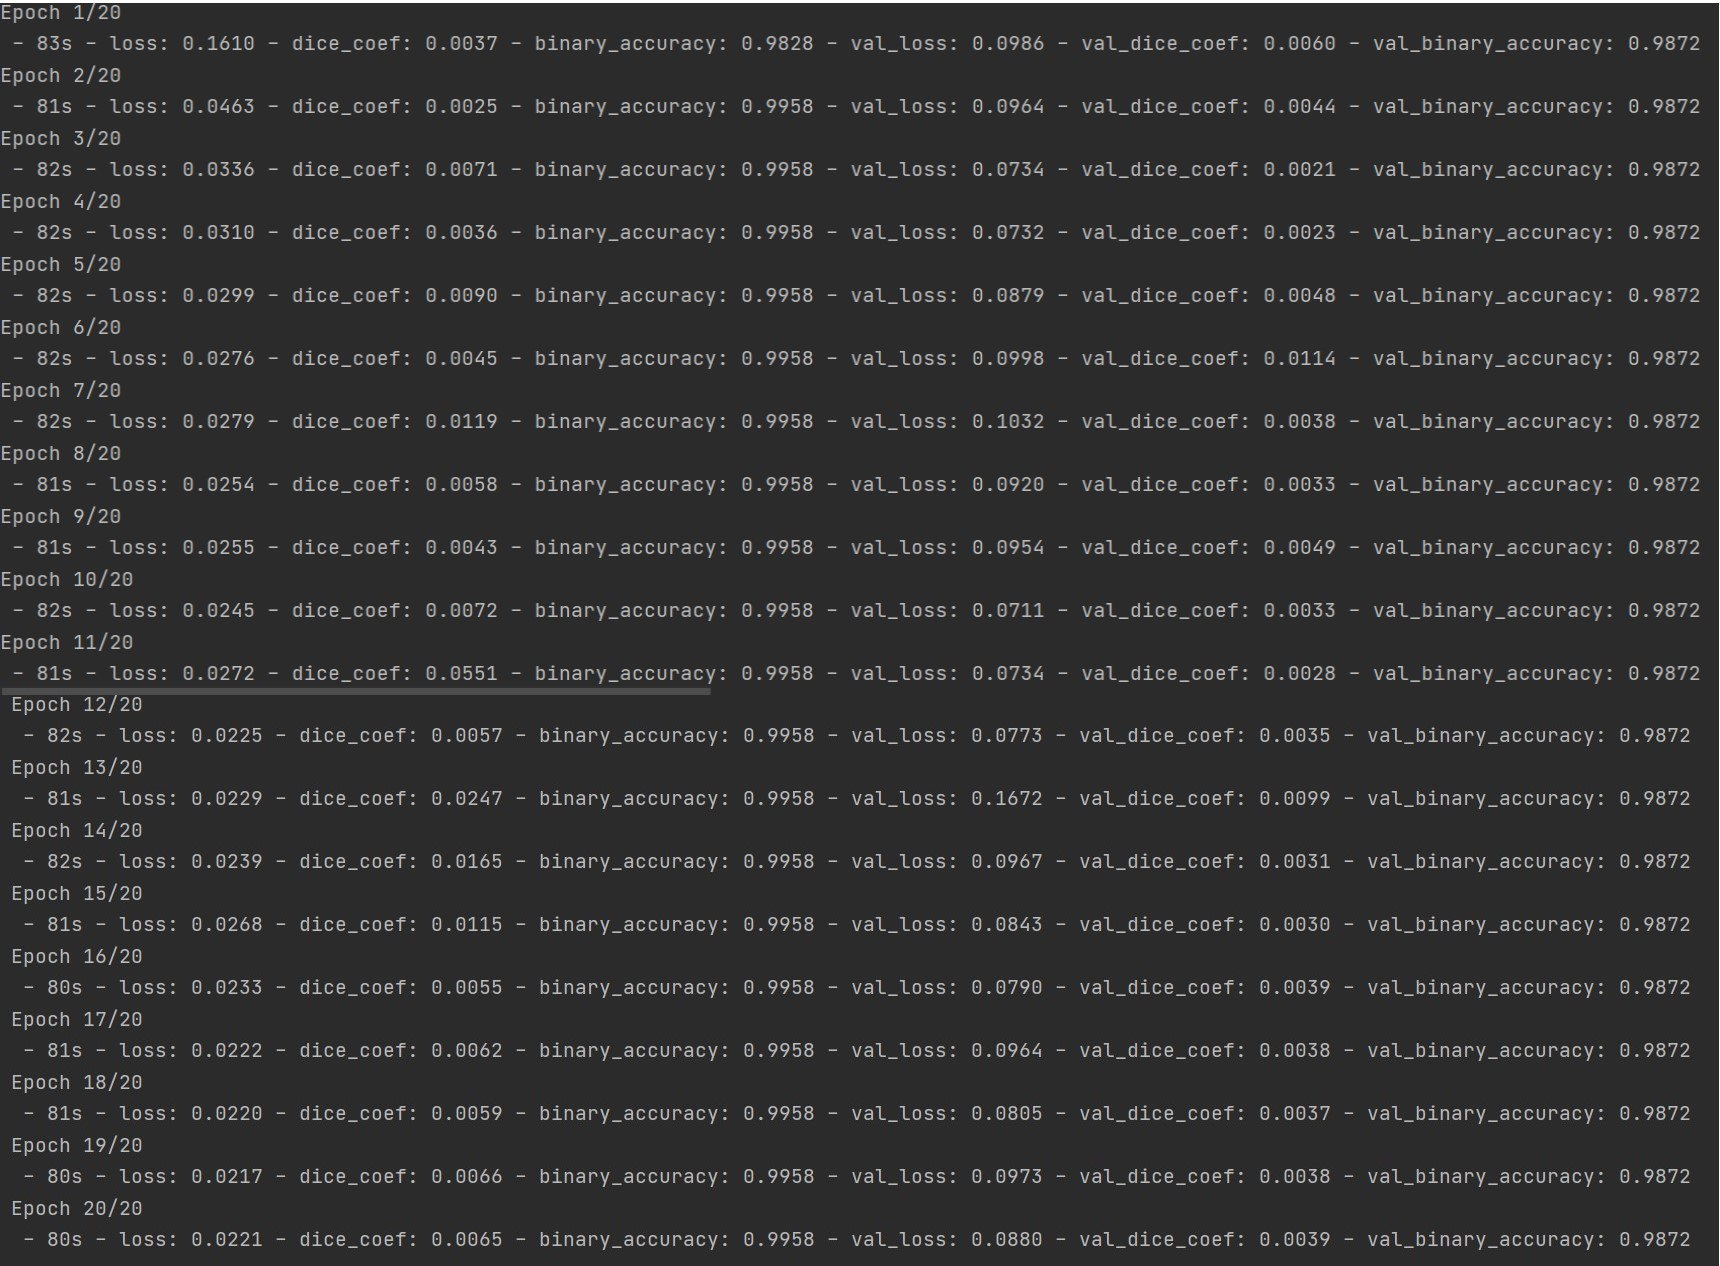
\includegraphics[width=15cm, height=10cm]{images/logs.jpg}}
	\caption{Logs}
	\label{logs}
\end{figure}

\section{Discussion}
\label{section:discussion}

As seen before, the results are quite disappointing. The UNets didn't manage to learn and identify, neither the prostate, nor the cancer area. The first reason this could happen may be the data. The input images are very dark, with a lot of noise and just a small part of them represents the prostate and even a smaller one describes the cancer area. The second reason may be the resize that is applied on every image. This operation reduces the quality of the data, making harder for the neural network to learn where the prostate or the cancer zone may be. Other reason that may explain these results could be the small amount of data. The data sets consists of only 890 slices. Moreover, the first and the last slices of every patient are very dark and the prostate area is very small. Due the hardware limitations, the hyper-parameters had to be adjusted accordingly. The batch size = 2, which may also have contributed to these results.


\chapter{Conclusion and future work}
\label{chapter:concl}

In this paper, we proposed and compared two U-Net models to accurately segment the prostate MRI. The hyperparameters are the same for both the U-Net, but the architecture is different. By using this 2 models, we were able to compare and analyze how the architecture of a neural network and the number of features can influence the performance, the accuracy and the speed of the learning process.\par
As we seen before, one of the greatest challenge we had to face was the input. The data set contained only 900 slices which had to be divided for training, validation and testing. Moreover, the images were dark, the prostate area was very small and each slice had to be resized at half of its normal size. All this made the learning process more difficult, which resulted in the U-Net to have problems while learning to detect the cancer zone. To overcome all these problems, we tried to improve the input data set using the data augmentation strategy and applying transformations such as translation, rotation and zoom.\par
Even if the results are not very satisfying and the U-Net models are not yet able to detect the prostate cancer zone very accurately, they still prove that a U-Net can be used for prostate cancer segmentation. With more training time and more competent hardware, if the number of epochs and the batch size is increased, as well as the original size of the input images is kept, and a better preprocessing of the input data, the result may improve and the models will be able to accurately detect the prostate cancer zone.\par
With all these improvements, and the intelligent algorithm included in the web application, the resulted software will be very helpful for a student that wants to study the prostate and the possible tumor zones. But, it is very important to keep in mind that, even if the model has learned to detect the prostate cancer zone very well, errors still may occur. Therefore, it is recommended to use AI as a complimentary evaluation and interpretation system, without relying solely on model-based decisions.

\bibliographystyle{plain}
\bibliography{bibliography.bib}
\end{document}